\documentclass[11pt,a4paper]{article}
\usepackage[T1]{fontenc}
\usepackage[utf8]{inputenc}
\usepackage{lmodern}
\usepackage{amsmath,amssymb,booktabs,array,graphicx,microtype}
\usepackage[margin=2.25cm]{geometry}
\usepackage[colorlinks=true,linkcolor=blue!55!black,citecolor=blue!55!black,urlcolor=blue!60!black]{hyperref}
\usepackage{xcolor}
\usepackage{enumitem}
\usepackage{caption}
\usepackage{float}
\usepackage{authblk}

\graphicspath{{outputs_paper76_state_conditioned_execution/}}
\newcommand{\Rrob}{R_{\rm rob}}
\newcommand{\Ggate}{G_{\rm gate}}
\newcommand{\MOMS}{\mathrm{MOMS}}
\newcommand{\eps}{\varepsilon}

\title{State-Conditioned Gate Arbitration in SAT/CDCL\\
\large Execution of the Preregistered MAAT v1.8 Gate Challenge Cycle II}
\author{Christof Krieg}
\affil{MAAT Project, Independent Researcher\\
\href{https://maat-research.com}{maat-research.com}}
\date{2026}

\begin{document}
\maketitle

\begin{abstract}
Paper 75 preregistered a state-conditioned SAT/CDCL arbitration protocol before
external execution and archived it at Zenodo
(DOI: \href{https://doi.org/10.5281/zenodo.21767033}{10.5281/zenodo.21767033}).
This paper executes that frozen protocol on 98 hashed SATLIB instances: 19
calibration instances and 79 held-out test instances across six families.  No
support equation, threshold, policy coefficient, split, budget, null model,
bootstrap rule, or status criterion was changed after preregistration.

The construction passes the frozen distinctness precondition and is not
reconstructed by the declared classical summary model.  Its realised
family--instance-weighted test activation is $0.12558$, narrowly above the
minimum $q_{\rm test,min}=0.125$.  Operationally, however, the result is
negative.  Against MOMS, the primary state-conditioned policy has
family-balanced total-cost difference
$\Delta U=-642.96$ with 95\% bootstrap interval
$[-841.63,-295.82]$, where positive values favour the state-conditioned
policy.  Relative regret against MOMS is $0.9135$
($95\%$ interval $[0.6956,1.1756]$), satisfying the preregistered definition
of \texttt{harmful}.  The primary policy also loses significantly to the
static v1.7 gate and score-with-$R$ baselines.  It beats the shuffled-gate null
but not the matched-random-activation null.  The frozen status tuple is
therefore
\texttt{executed / distinct / adequate\_activation / harmful /
negative\_result}.  A secondary decomposition shows that structural overhead
amplifies the failure, but search cost alone also loses to MOMS.  This is a
negative external execution result, not a retuned gate proposal.
\end{abstract}

\section{Purpose and Release Barrier}

The question is whether structural supports evaluated on the evolving CDCL
state can arbitrate usefully between a structural Mode-A brancher and a
classical MOMS fallback.  Paper 75 fixed the complete experiment before any
external state-conditioned run.  The exact release was published on 3 August
2026 as version 1.5.3 and assigned DOI
\href{https://doi.org/10.5281/zenodo.21767033}{10.5281/zenodo.21767033}.
Paper 76 began only after that public timestamp.

Three immutable identifiers guard the execution:
\begin{align*}
\text{Paper-75 DOI}&=\texttt{10.5281/zenodo.21767033},\\
\text{protocol SHA256}&=\texttt{9e86b1e1f8ddcd3228c90f62cc9465d3}\ldots,\\
\text{manifest SHA256}&=\texttt{941fad18c5ea4839ee3aac4b5d7f1e3d}\ldots.
\end{align*}
The external gatekeeper also required all 98 raw-file hashes, DIMACS
parseability, and absence of unknown CNFs to pass.  All checks passed before
the solver was called.

\section{Frozen Protocol}

This section summarises the executed contract; the preregistration remains the
authoritative specification~\cite{krieg75}.

\subsection{Decision state and supports}

Supports are evaluated after unit propagation reaches a conflict-free fixpoint
and immediately before each branch decision.  The state contains original and
persistent learned clauses, the partial assignment, decision levels, trail,
reason clauses, VSIDS activity, and saved phase.  Satisfied clauses are removed
and falsified literals are deleted to form the residual CNF $F_t$.

On active residual variables $U_t$, the frozen supports are
\begin{align}
H[X_t]&=\left(1+\operatorname{mean}_{v\in U_t}
\frac{|p_v-n_v|}{p_v+n_v+10^{-9}}\right)^{-1},\\
B[X_t]&=\left(1+\frac{\operatorname{std}_{v\in U_t}(d_v)}
{\operatorname{mean}_{v\in U_t}(d_v)+10^{-9}}\right)^{-1},\\
S[X_t]&=\frac{\operatorname{mean}_{v\in U_t}(s_v)}
{\max_{v\in U_t}s_v+10^{-9}},\\
V[X_t]&=\operatorname{clip}_{[0,1]}
\left(0.65f_{\rm LCC}+0.35\bar c\right).
\end{align}
Here $p_v,n_v$ are residual positive and negative occurrence counts,
$d_v=p_v+n_v$, $s_v$ is inverse-length-weighted pressure from residual
clauses of length at most three, $f_{\rm LCC}$ is the largest component
fraction, and $\bar c$ is mean local clustering.  The emergent closure is
\begin{equation}
\Rrob=\min\left((HBV)^{1/3},(HBSV)^{1/4}\right).
\end{equation}

\subsection{Calibration and arbitration}

Only MOMS trajectories from the 19 calibration instances determine weighted
medians, MADs, the gate threshold, tie fraction, distinctness, and classical
reconstruction.  At most 128 deterministically selected states are retained
per instance; 667 states were retained in this execution.  The primary gate is
\begin{equation}
g_t=z_R+0.50z_t,\qquad \Ggate=(1+e^{-g_t})^{-1}.
\end{equation}
The weighted lower $0.75$ quantile produced
\begin{equation}
\theta_q=0.8816963,\qquad f_{\rm tie}=0.7287115.
\end{equation}
The calibration median and MAD were $0.7627958$ and $0.0446364$ for
$\Rrob$, and $-0.0018129$ and $0.0089476$ for $\Delta\Rrob$.

The gate routes to Paper-63 Mode A when active and to MOMS otherwise.  Mode A
uses the frozen candidate score
\begin{equation}
A_t(v)=P_t(v)-0.38h_{\rm MAAT,t}(v)
\end{equation}
with softmax inverse temperature $8$.  Directly compared stochastic policies
use the same state-bound random number whenever they reach the same state.

\subsection{Causal updates and overhead}

The implementation maintains residual literal counts, short-clause pressure,
and graph-edge multiplicities incrementally.  Enqueue operations update the
counters; assignment effects are reversed on backtrack; learned clauses remain
persistent.  Every 100th decision compares incremental supports against full
reconstruction.  The maximum discrepancy observed in the complete run was
$7.27\times10^{-14}$, below the frozen $10^{-12}$ abort tolerance.

Each policy-instance pair has 5000 conflicts and 30 seconds.  Search cost is
\begin{equation}
C_{\rm search}=N_{\rm conflict}+0.30N_{\rm decision}
+0.004N_{\rm propagation}+5000\mathbf1[\mathrm{timeout}].
\end{equation}
Calibration fixed $\kappa_{\rm cal}=268.943$ search-cost units per second.
For structural policies,
\begin{equation}
C_{\rm total}=C_{\rm search}+\kappa_{\rm cal}T_{\rm structural}.
\end{equation}
Classical baselines report tracing timers separately but are not charged for
diagnostic work that their decision rules do not require.

\section{Data and Gatekeeper}

The manifest contains AIM (20), Dubois (13), pigeonhole (5), flat graph
colouring (20), satisfiable random 3-SAT UF20 (20), and unsatisfiable random
3-SAT UUF50 (20), sourced from SATLIB~\cite{satlib}.  Frozen family-local
hash ordering assigns 19 instances to calibration and 79 to testing.

\begin{table}[H]
\centering
\caption{Pre-execution gatekeeper.}
\begin{tabular}{lc}
\toprule
Check & Status\\
\midrule
Published Paper-75 release and DOI & PASS\\
Protocol and manifest SHA256 & PASS\\
98 expected CNFs present & PASS\\
98 instance SHA256 values & PASS\\
DIMACS parseability & PASS\\
No unexpected CNFs & PASS\\
\bottomrule
\end{tabular}
\end{table}

Raw SATLIB CNFs are not redistributed.  Only source metadata, hashes, and
derived solver measurements are included with the experiment.

\section{Construct and Activation Status}

No support pair approached the frozen degeneracy boundary
$|\rho_S|>0.99$.  The largest absolute weighted Spearman correlation was
$0.6821$ between $B$ and $S$; weighted support standard deviations ranged from
$0.0769$ to $0.1507$.  The construct therefore passed distinctness.

The preregistered 18-predictor classical reconstruction produced negative
held-out weighted $R^2$ for all targets, including $\Rrob$ and $\Ggate$.
These very negative values indicate unstable extrapolation by the declared OLS
model, not ``negative predictability.''  They are nevertheless below the
frozen convergent-rediscovery threshold $0.90$, so
\texttt{construct\_status=distinct}.

Family--instance-weighted activation was $0.1255808$.  This narrowly exceeds
the predeclared minimum $q_{\rm test,min}=0.125$ while remaining far below the
calibration target $q=0.25$.  Accordingly,
\texttt{activation\_status=adequate\_activation}; the proximity to the boundary
is reported without threshold adjustment.

\begin{figure}[H]
\centering
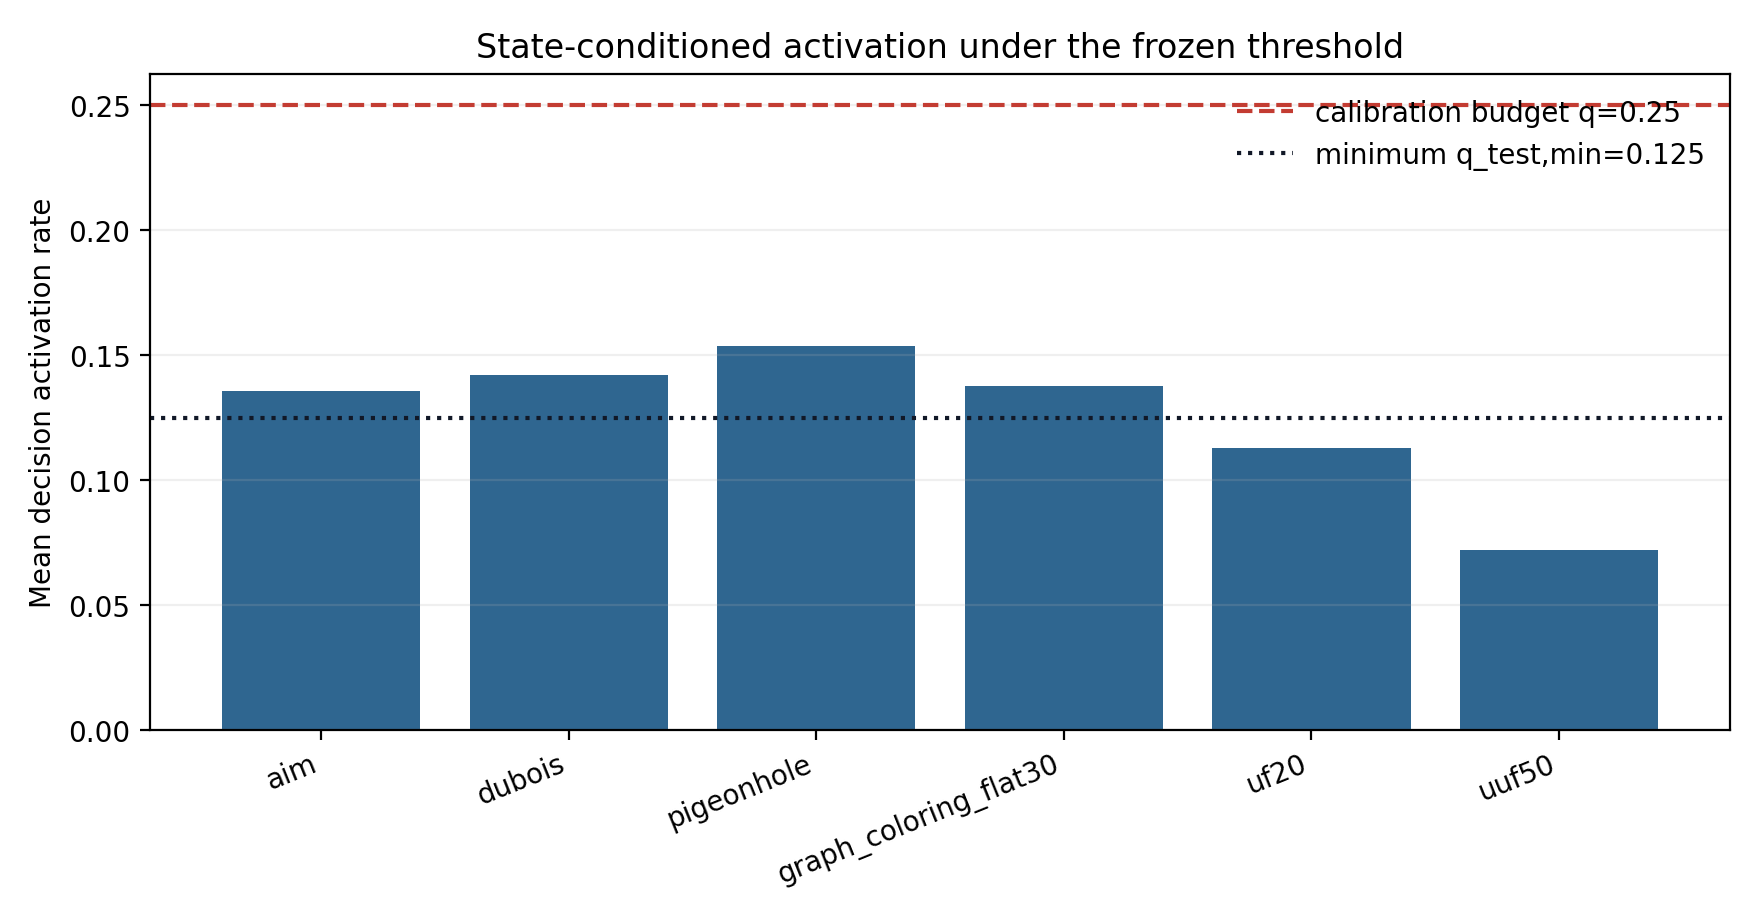
\includegraphics[width=0.89\linewidth]{fig4_activation_by_family.png}
\caption{Realised primary activation by family.  The frozen threshold is not
refitted on test states.}
\end{figure}

\section{Primary Utility Results}

For policy $A$ against comparator $B$, the registered direction is
\begin{equation}
\Delta U_i(A,B)=C_B(i)-C_A(i),
\end{equation}
so positive values favour the state-conditioned policy.  Confidence intervals
use 10,000 paired instance-level bootstrap resamples within family followed by
equal family aggregation.

\begin{table}[H]
\centering
\caption{Primary state-v1.8 comparisons.  Wins and losses refer to the primary
policy; means and intervals are family-balanced.}
\small
\begin{tabular}{lrrrr}
\toprule
Comparator & Mean $\Delta U$ & 95\% CI & Wins & Losses\\
\midrule
Static v1.7 gate & -517.20 & [-704.89, -177.72] & 54 & 25\\
Score-with-$R$ & -522.90 & [-715.03, -172.41] & 53 & 26\\
Shuffled gate & 42.24 & [6.65, 70.14] & 43 & 36\\
Matched random activation & 23.96 & [-8.27, 51.14] & 46 & 33\\
MOMS & -642.96 & [-841.63, -295.82] & 5 & 74\\
Jeroslow--Wang & -533.75 & [-727.05, -209.60] & 35 & 44\\
VSIDS & -862.58 & [-1605.14, -274.01] & 47 & 32\\
\bottomrule
\end{tabular}
\end{table}

The apparent contrast between majority wins against the two prior MAAT
baselines and strongly negative family-balanced means is a tail effect: fewer,
costly losses dominate the average.  Against MOMS the primary policy wins only
five of 79 paired test cases.

\begin{figure}[H]
\centering
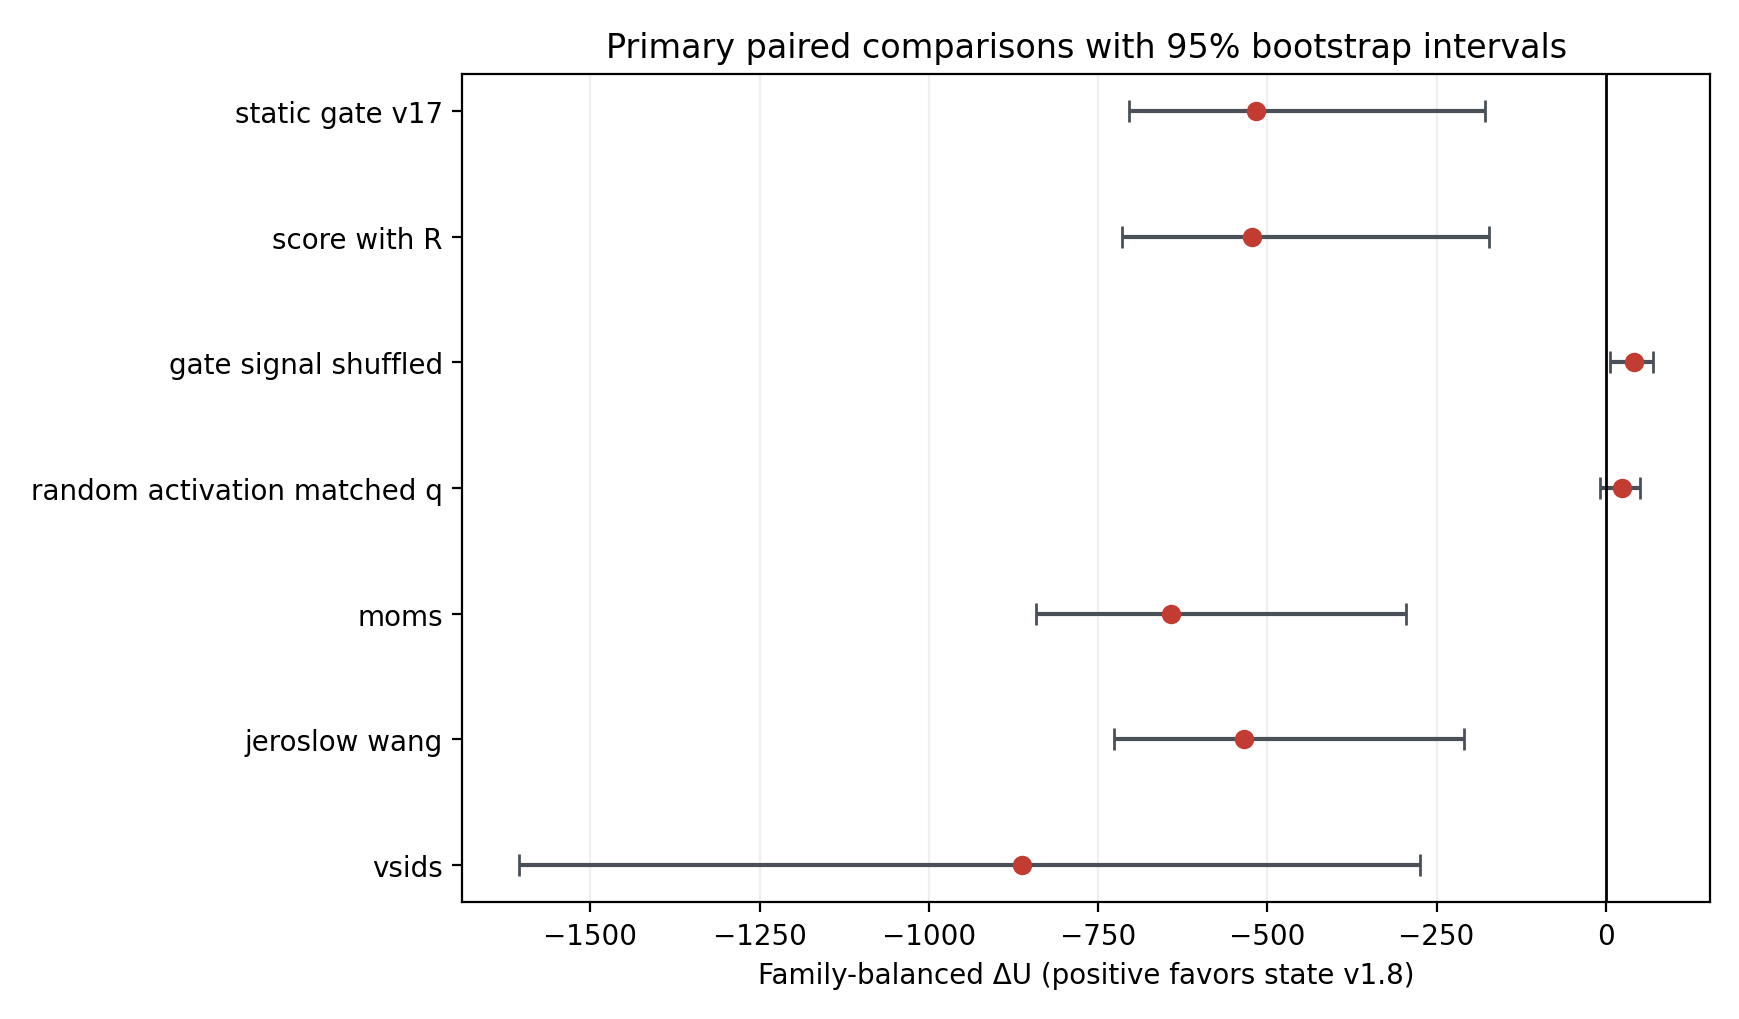
\includegraphics[width=0.92\linewidth]{fig2_primary_comparisons.png}
\caption{Primary paired comparisons.  Positive values favour state v1.8.}
\end{figure}

The primary policy significantly beats the shuffled-gate null, showing that
the realised gate sequence is not equivalent to the declared family/split
shuffle.  It does not significantly beat matched random activation.  The
minimum-support rule requires positive lower confidence bounds against both
prior MAAT baselines and both nulls; it is therefore not met.

\section{Safety and Cost Decomposition}

Relative regret against the frozen MOMS fallback is
\begin{equation}
r_i=\frac{C_{\rm state}(i)-C_{\MOMS}(i)}{\max(C_{\MOMS}(i),10^{-9})}.
\end{equation}
The family-balanced mean is $0.91349$ with interval
$[0.69560,1.17557]$.  Because the lower endpoint exceeds the frozen no-harm
bound $\delta=0.05$, the registered safety label is
\texttt{harmful}.  This is positive evidence of harm under the registered cost
model, not merely failure to certify no harm.

A secondary, non-reclassifying decomposition separates search decisions from
charged structural overhead.  Against MOMS, search cost alone yields
$\Delta U=-49.42$ with interval $[-69.81,-30.82]$.  Total cost yields
$-642.96$ with interval $[-841.63,-295.82]$.  Mean measured structural overhead
for the primary policy is $0.7054$ seconds per test instance.  Thus overhead is
the dominant damage channel, especially on timeout trajectories, but removing
it would not reverse the negative search result.

\begin{table}[H]
\centering
\caption{Descriptive family means versus MOMS.  Positive deltas favour state
v1.8; this table does not alter the preregistered classification.}
\small
\begin{tabular}{lrrr}
\toprule
Family & Search $\Delta U$ & Total $\Delta U$ & Overhead penalty\\
\midrule
AIM & 0.67 & -7.41 & 8.08\\
Dubois & -275.44 & -348.66 & 73.22\\
Pigeonhole & -18.51 & -3487.42 & 3468.91\\
Flat30 & 0.00 & -1.40 & 1.40\\
UF20 & -0.11 & -0.57 & 0.46\\
UUF50 & -3.10 & -12.31 & 9.21\\
\bottomrule
\end{tabular}
\end{table}

\begin{figure}[H]
\centering
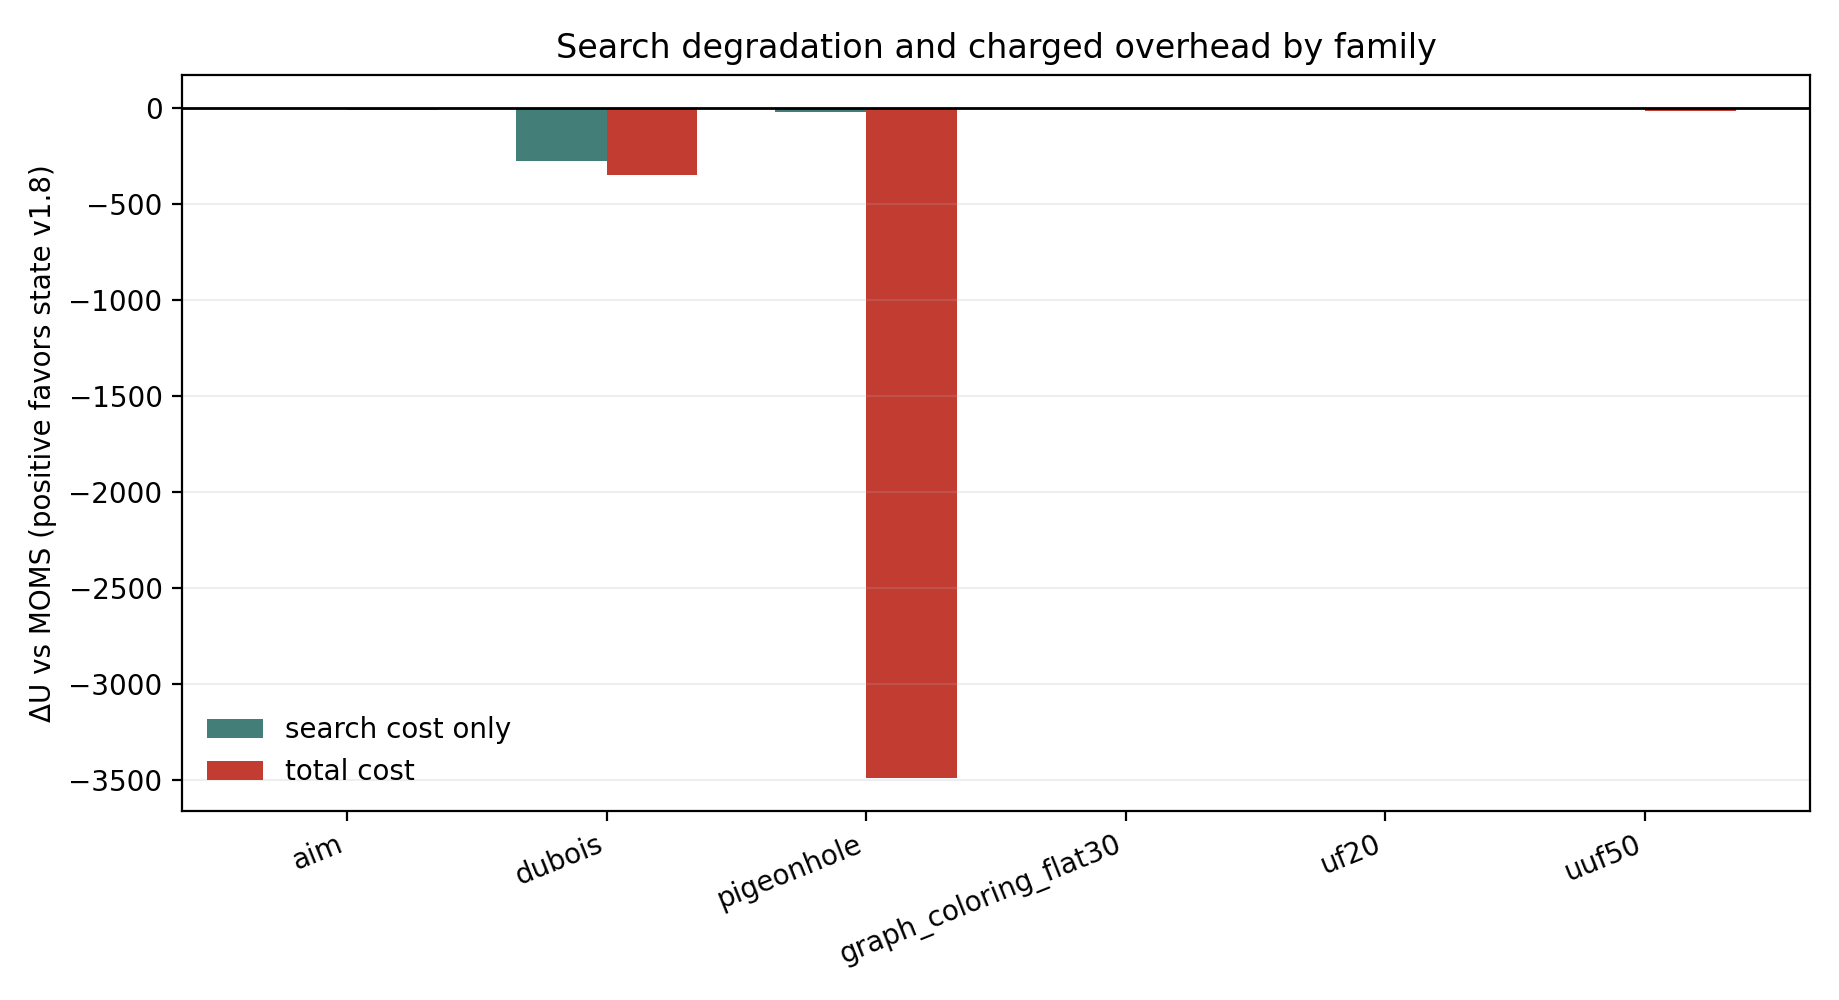
\includegraphics[width=0.92\linewidth]{fig3_family_cost_decomposition.png}
\caption{Search-only and overhead-inclusive family deltas versus MOMS.  The
pigeonhole tail dominates charged overhead, while Dubois also exhibits genuine
search degradation.}
\end{figure}

\section{Complete Frozen Outcome}

Paper 75 requires independent status axes rather than a single favourable or
unfavourable label.

\begin{table}[H]
\centering
\caption{Paper-76 outcome under the frozen status system.}
\begin{tabular}{ll}
\toprule
Axis & Frozen result\\
\midrule
Execution & \texttt{executed}\\
Construct & \texttt{distinct}\\
Activation & \texttt{adequate\_activation}\\
Safety & \texttt{harmful}\\
Utility & \texttt{negative\_result}\\
\bottomrule
\end{tabular}
\end{table}

The negative utility label follows independently from the confidence intervals
against static v1.7 and score-with-$R$.  The harmful safety label follows from
relative regret against MOMS.  Passing distinctness and activation does not
override either result.

\section{Interpretation}

The experiment rejects the practical utility of this frozen state-conditioned
arbitration on the declared benchmark.  It does not imply that every dynamic
SAT state descriptor is useless, nor does it test an industrial solver.  It
does show that three appealing properties---nondegenerate supports, a
nontrivial gate, and partial superiority to a shuffled null---are insufficient
for decision utility.

Two failures coexist.  First, Mode-A activation degrades search in important
families, most clearly Dubois.  Second, continuously maintaining residual graph
and support information is expensive on long timeout trajectories.  A fallback
architecture cannot claim safety merely because it activates infrequently:
here activation barely clears the registered minimum yet still produces a
harmful relative-regret interval.

No threshold, support, data split, budget, or status rule is modified in this
paper.  Any future attempt to reduce graph-update overhead or alter the active
policy would constitute a new hypothesis and require a new preregistration.

\section{Limitations}

\begin{itemize}[leftmargin=1.5em]
\item The transparent Python CDCL backend is auditable but not an industrial
solver such as CaDiCaL or Kissat.  Results concern policy comparison within this
shared backend.
\item The benchmark contains six public SATLIB families but only 98 instances.
The pigeonhole family has four test cases and therefore yields uncertain tail
estimates despite equal-family aggregation.
\item The OLS reconstruction model extrapolates poorly.  Its negative $R^2$
values satisfy the frozen non-reconstruction condition but do not establish a
strong positive notion of structural novelty.
\item Runtime depends on the execution environment.  The primary registered
cost converts measured overhead using calibration-derived $\kappa_{\rm cal}$;
raw wall time and operation-count search cost are both retained.
\item Secondary ablations are descriptive only.  None may replace the failed
primary policy or promote its status.
\end{itemize}

\section{Data, Licensing, and Reproducibility}

Repository:
\begin{center}
\url{https://github.com/Chris4081/structural-selection-principle}
\end{center}
Experiment folder:
\begin{center}
\texttt{experiments/maat\_v18\_state\_conditioned\_execution\_paper76/}
\end{center}
The release includes code, the frozen metadata manifest, validation JSON,
derived CSV/JSON outputs, figures, tests, and this manuscript.  Raw SATLIB CNFs
and source archives are intentionally excluded.  Users must obtain them from
SATLIB and verify them against the included SHA256 manifest.  SATLIB authors
and maintainers do not endorse MAAT.

Paper 76, its figures, and the derived result tables are released under the
Creative Commons Attribution 4.0 International license (CC BY 4.0).  Repository
source code remains under the MIT License.  Paper 75 is likewise archived under
CC BY 4.0 on Zenodo.  External SATLIB benchmark materials are not included and
retain their original terms.  The manifest provides attribution, source URLs,
and integrity metadata but grants no additional rights in those external
instances.  The derived output tables contain solver measurements and metadata,
not clause lists.

Reproduction begins with
\begin{verbatim}
python3 paper76_execution.py --data-dir /path/to/data_external --validate-only
\end{verbatim}
and proceeds only after \texttt{VALIDATION PASS}.  The complete run is
\begin{verbatim}
python3 paper76_execution.py --data-dir /path/to/data_external
python3 paper76_report.py
\end{verbatim}
Synthetic unit tests are executed with
\begin{verbatim}
PYTHONDONTWRITEBYTECODE=1 python3 -m unittest discover -s tests -v
\end{verbatim}

\section{Conclusion}

Paper 76 completes the first execution of MAAT v1.8 Gate Challenge Cycle II.
The experiment passed release, data, implementation, distinctness, and minimum
activation checks.  It nevertheless produced a harmful safety result and a
negative utility result.  The frozen state-conditioned gate is therefore not
supported as a practical SAT/CDCL improvement under this protocol.

This outcome is accepted without modifying the preregistered hypothesis.

\begin{thebibliography}{9}
\bibitem{krieg75}
C. Krieg, ``State-Conditioned Gate Arbitration in SAT/CDCL: A
Preregistration for MAAT v1.8 Gate Challenge Cycle II,'' Paper 75 (2026),
\url{https://doi.org/10.5281/zenodo.21767033}.

\bibitem{satlib}
H. H. Hoos and T. St\"utzle, ``SATLIB: An Online Resource for Research on
SAT,'' in \emph{SAT 2000}, IOS Press (2000),
\url{https://www.cs.ubc.ca/~hoos/SATLIB/}.

\bibitem{moms}
J. N. Hooker and V. Vinay, ``Branching Rules for Satisfiability,''
\emph{Journal of Automated Reasoning} \textbf{15}, 359--383 (1995).

\bibitem{jw}
R. G. Jeroslow and J. Wang, ``Solving Propositional Satisfiability Problems,''
\emph{Annals of Mathematics and Artificial Intelligence} \textbf{1},
167--187 (1990).

\bibitem{chaff}
M. W. Moskewicz \emph{et al.}, ``Chaff: Engineering an Efficient SAT Solver,''
in \emph{DAC 2001}, 530--535 (2001).
\end{thebibliography}

\end{document}
